\documentclass[conference]{IEEEtran}
\usepackage{cite}
\usepackage{amsmath,amssymb}
\usepackage{booktabs}
\usepackage{graphicx}
\usepackage{url}
\usepackage{xcolor}
\usepackage{array}
\graphicspath{{figures/}}
\newcommand{\code}[1]{\texttt{#1}}
\begin{document}

\title{Layer-Contrastive Decoding and Epistemic Reliability Estimation for Hallucination-Aware Small Language Models}

\author{\IEEEauthorblockN{E. Ganesh Kumar Reddy, B. Sai Susmitha, P. Dhanush Datta, and E. Sri Vardhan Reddy}
\IEEEauthorblockA{School of Computer Science and Engineering (SCOPE), VIT-AP University, Amaravati, India\\
Project Guide: Palacharla Ravi Kumar, Assistant Professor Sr. Grade-2}}
\maketitle

\begin{abstract}
Small language models can produce fluent answers that are unsupported or false; token likelihood is not, by itself, a calibrated measure of answer-level reliability. This paper audits a TinyLlama-1.1B pipeline that combines Decoding by Contrasting Layers (DoLa), an Epistemic Neural Network (ENN), and sampled self-consistency. The active implementation extracts mature and dynamically selected premature hidden states, contrasts their vocabulary logits, trains a frozen-prior epinet for next-token prediction on document-disjoint C4 features, and optionally aggregates sampled answers. The repository also retains results from an upgraded, answer-correctness ENN benchmark. Those results are analyzed separately because the corresponding trainer is absent from the active checkout. On the archived 211-example held-out set (169 TruthfulQA and 42 HaluEval-QA examples; 54 positive and 157 negative labels), the 2048-dimensional ENN representation achieved AUROC 0.691, AUPRC 0.513, and accuracy 0.782. At a conservative calibrated operating point, DoLa+ENN achieved accuracy 0.768, precision 0.647, recall 0.204, F1 0.310, ECE 0.123, and a false-accept rate of 0.038. Adding self-consistency left these decisions unchanged. McNemar's test found a significant difference between DoLa and DoLa+ENN, but not between DoLa+ENN and the complete combined architecture. The findings support uncertainty-aware abstention rather than a general claim of hallucination prevention. Missing upgraded source files and class-imbalance-sensitive thresholding constrain reproducibility and generalization.
\end{abstract}

\begin{IEEEkeywords}
large language models, hallucination detection, factuality, DoLa, epistemic neural networks, uncertainty estimation, self-consistency, calibration
\end{IEEEkeywords}

\section{Introduction}
Large language models (LLMs) have made autoregressive generation useful for question answering, summarization, and interactive assistance. Their training objective, however, rewards continuation likelihood rather than truth. A model can therefore produce a coherent answer that conflicts with evidence or encodes a common misconception. TruthfulQA formalized this problem with questions designed to elicit false beliefs from language models~\cite{lin2022truthfulqa}; HaluEval broadened evaluation with human-annotated hallucinated and normal samples~\cite{li2023halueval}. Hallucination detection asks whether an output is unreliable. Hallucination mitigation changes the generation or selection process so that unreliable outputs become less likely. The two operations are related but not equivalent.

This capstone examines a reliability pipeline centered on TinyLlama-1.1B-Chat-v1.0~\cite{zhang2024tinyllama}. The active code implements (i) layer-contrastive decoding, (ii) a PyTorch epinet trained on C4 next-token features, (iii) plurality and entropy-weighted self-consistency, and (iv) evaluation and plotting utilities. DoLa contrasts later and earlier layer distributions so that information emerging in deeper layers can influence decoding~\cite{chuang2024dola}. ENNs define joint predictions through a sampled epistemic variable~\cite{osband2021enn}. Self-consistency aggregates multiple sampled reasoning paths~\cite{wang2023selfconsistency}.

The repository also preserves a later audit package reporting answer-correctness ENN variants. Its results are valuable, but the corresponding Python source is not present: only compiled remnants, checkpoints, plots, and reports remain. We therefore distinguish implementation facts directly verified from the active source from empirical findings archived by the project. This distinction prevents a common failure mode in research reporting: describing a stronger historical artifact as though it were the current executable system.

The contributions are: (1) a complete, mathematical description of the active TinyLlama--DoLa--Epinet pipeline; (2) a separation of token-level uncertainty, answer-level detection, and decoding mitigation; (3) a code-grounded analysis of the archived held-out benchmark, including operating-point trade-offs, ablations, confidence intervals, and paired tests; and (4) a reproducibility audit identifying exactly which conclusions are supported and which require recovery of missing source or new runs.

\section{Related Work}
\subsection{Hallucination and factuality}
Hallucination has multiple operational definitions, including conflict with external facts, lack of support from a source, and inconsistency with instructions or context. TruthfulQA evaluates truthfulness under misconception-inducing questions~\cite{lin2022truthfulqa}; HaluEval provides a larger hallucination-recognition benchmark~\cite{li2023halueval}. Recent audits emphasize that reported scores depend strongly on task definition and annotation protocol~\cite{ji2023survey,huang2024audit}.

\subsection{Decoding and self-consistency}
DoLa uses contrast between mature and premature layer distributions and reports factuality gains without fine-tuning the base model~\cite{chuang2024dola}. In this project, DoLa is implemented as a sparse per-position JSD-based selector over TinyLlama blocks. Self-consistency samples multiple outputs and selects the most consistent final answer~\cite{wang2023selfconsistency}; agreement improves stability in some reasoning settings but can also produce consistent errors.

\subsection{Uncertainty and calibration}
Epistemic neural networks augment a predictor with an epistemic index and are intended to represent uncertainty-sensitive joint predictions~\cite{osband2021enn}. The active project uses an epinet with a frozen random prior and a trainable indexed residual. Its native target is C4 next-token prediction, not answer correctness. Calibration must therefore be measured separately: confidence should reflect empirical correctness likelihood, as emphasized by Guo \emph{et al.}~\cite{guo2017calibration}. The archived upgrade changes the target to answer correctness and evaluates MC-dropout and deep-ensemble variants, but those trainer sources are missing from the current checkout.

\subsection{Research gap}
Prior work motivates DoLa, ENNs, and self-consistency individually, but does not establish performance for this TinyLlama implementation or for its two distinct ENN formulations. The project addresses an engineering and evaluation gap by making the components inspectable and by comparing their reliability behavior. The available artifacts do not support a claim of a universally superior hallucination-prevention method.

\section{Problem Formulation}
For a question or context $q$, the frozen causal model with parameters $\theta$ generates a token sequence $a=(a_1,\ldots,a_T)$. At position $t$, let $h_t^m$ be the mature hidden state and $h_t^p$ the selected premature state after the normalization used for LM-head projection, and let $W$ denote the LM-head matrix. DoLa computes
\begin{equation}
\ell_t^{D}=W h_t^m-\alpha W h_t^p,\qquad p_t^{D}=\operatorname{softmax}(\ell_t^{D}).
\label{eq:dola}
\end{equation}
For each candidate layer $j$, the implementation computes $p_t^j=\operatorname{softmax}(W\operatorname{norm}(h_t^j))$ and selects
\begin{equation}
j_t^*=\arg\max_{j\in\{0,4,8,12,16,20\}} \operatorname{JSD}(p_t^m\|p_t^j).
\label{eq:jsd}
\end{equation}
The mature block is 21 in the 22-block TinyLlama model. The active default is $\alpha=0.05$; it is a configuration value, not a reported optimum.

The active ENN receives $x_t=[h_t^m;h_t^p]\in\mathbb{R}^{4096}$ and an epistemic index $z\sim\mathcal{N}(0,I_6)$. A frozen prior branch $f_0$ and trainable branch $f_\phi$ produce 2048-dimensional residuals. The training objective is sampled next-token cross-entropy:
\begin{equation}
\begin{aligned}
\mathcal{L}(\phi)
&=\frac{1}{|\mathcal{D}|K}\sum_{(x_t,y_t)\in\mathcal{D}}\sum_{k=1}^{K}\\[-2pt]
&\quad \operatorname{CE}\left(\ell_t^D+W[f_0(x_t,z_k)+f_\phi(x_t,z_k)],y_t\right).
\end{aligned}
\label{eq:ennloss}
\end{equation}
At inference, sampled distributions $p_k$ yield predictive entropy $H(\bar p)$, expected entropy $K^{-1}\sum_kH(p_k)$, and the implemented nonnegative epistemic proxy $\max(0,H(\bar p)-K^{-1}\sum_kH(p_k))$. These are token-distribution quantities, not correctness probabilities.

For answer-level detection, let $r_i\in\{0,1\}$ indicate whether answer $i$ is reliable and $s_i$ be a model score. A threshold $\tau$ produces $\hat r_i=\mathbb{1}[s_i\geq\tau]$. We report accuracy, precision, recall, F1, AUROC, AUPRC, Brier score, ECE, false-accept rate (FAR), and false-reject rate (FRR). Mitigation is evaluated separately through candidate selection or decoding; a detector can reduce FAR by rejecting most answers while having poor recall.

\section{Proposed Methodology}
\subsection{System architecture}
Fig.~\ref{fig:architecture} distinguishes the active system from the archived answer-correctness upgrade. The base model remains frozen during active ENN training and inference. C4 features train the active epinet, whereas the question-answering path supports Base and DoLa generation, ENN scoring, and self-consistency.
\begin{figure}[t]\centering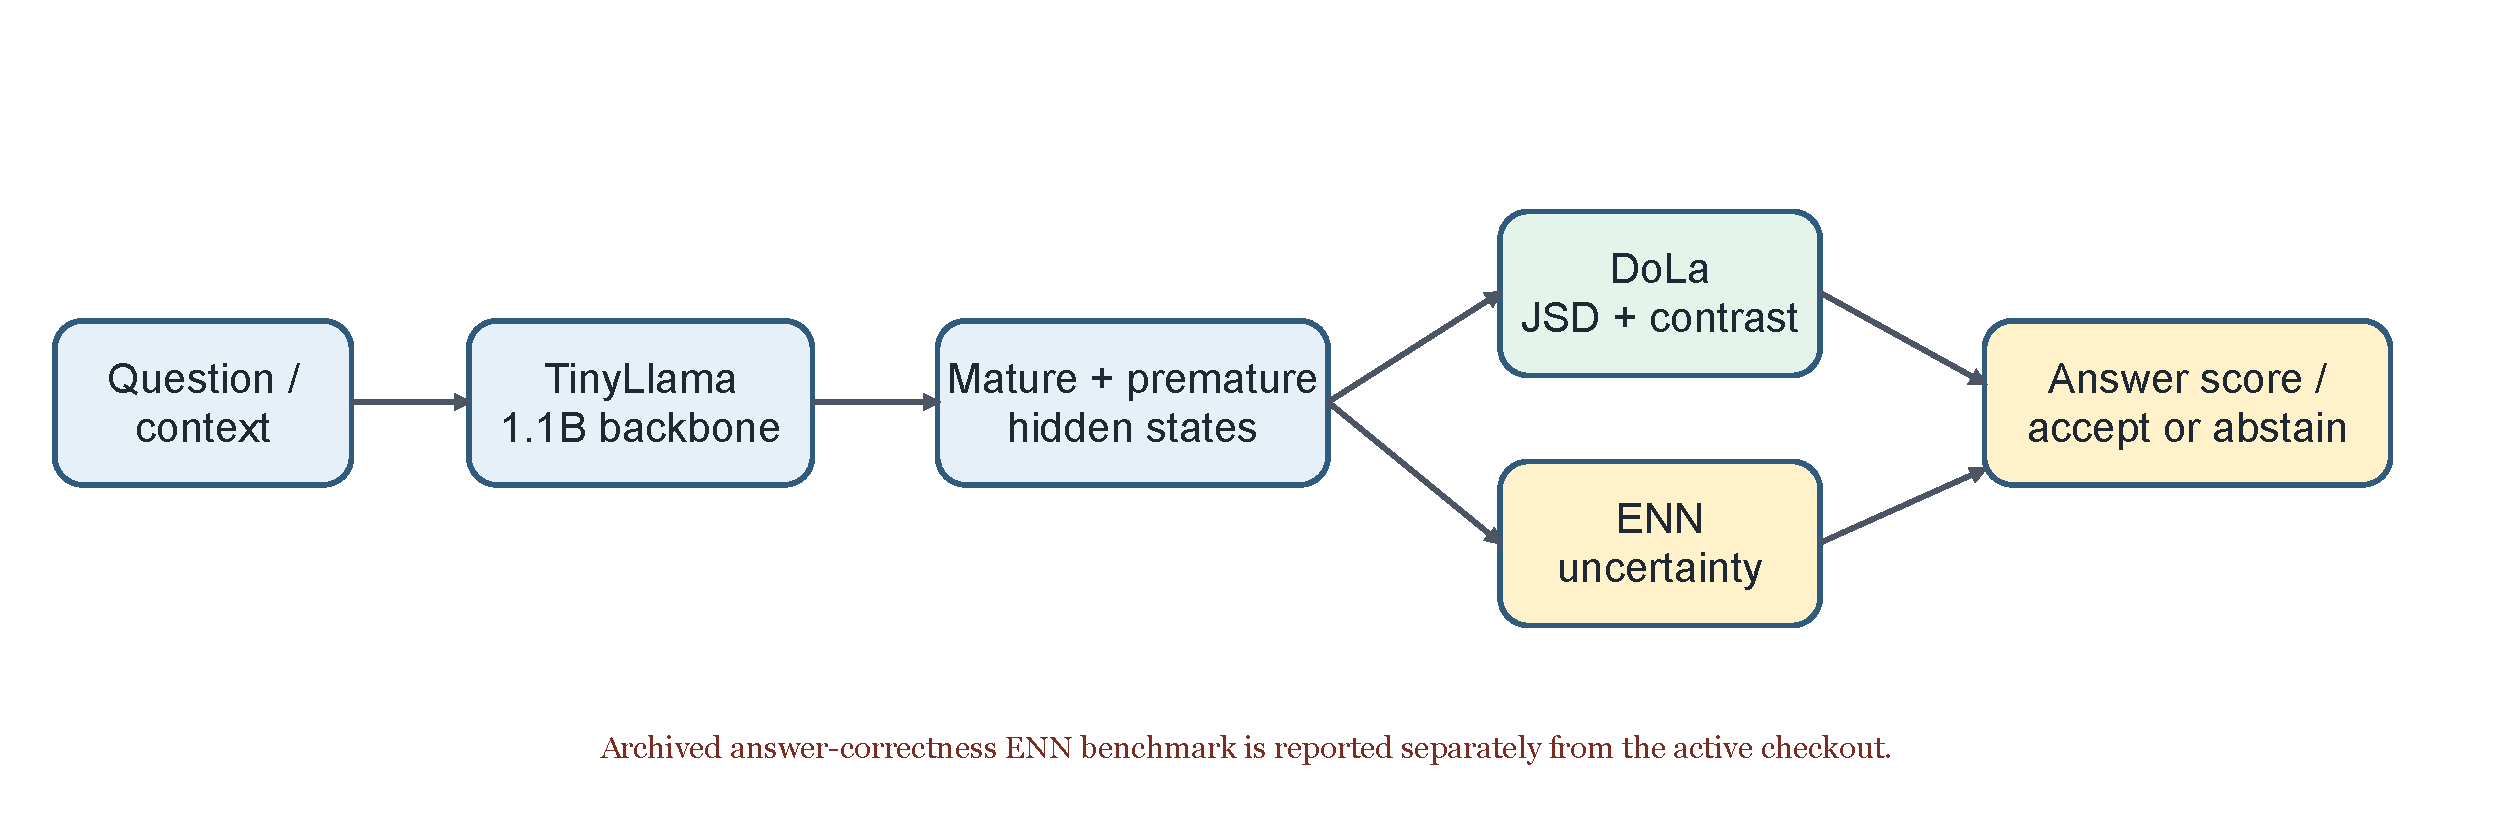
\includegraphics[width=\columnwidth]{Fig_1_Architecture.pdf}\caption{Active repository pipeline and the boundary to the archived upgraded benchmark.}\label{fig:architecture}\end{figure}

\subsection{Base language model and DoLa}
The repository loads a local TinyLlama-1.1B-Chat-v1.0 checkpoint through Hugging Face Transformers. The model has 22 transformer blocks, a hidden size of 2048, and a vocabulary of 32,000 tokens. DoLa obtains all hidden states in one forward pass, excludes the embedding output, applies the model RMS normalization to intermediate states, and projects each candidate through the LM head. It then contrasts the mature and selected premature logits as defined in (1). The implementation searches a sparse set of candidate layers rather than every layer; this is an implementation choice, not the full DoLa search.

\begin{figure}[t]\centering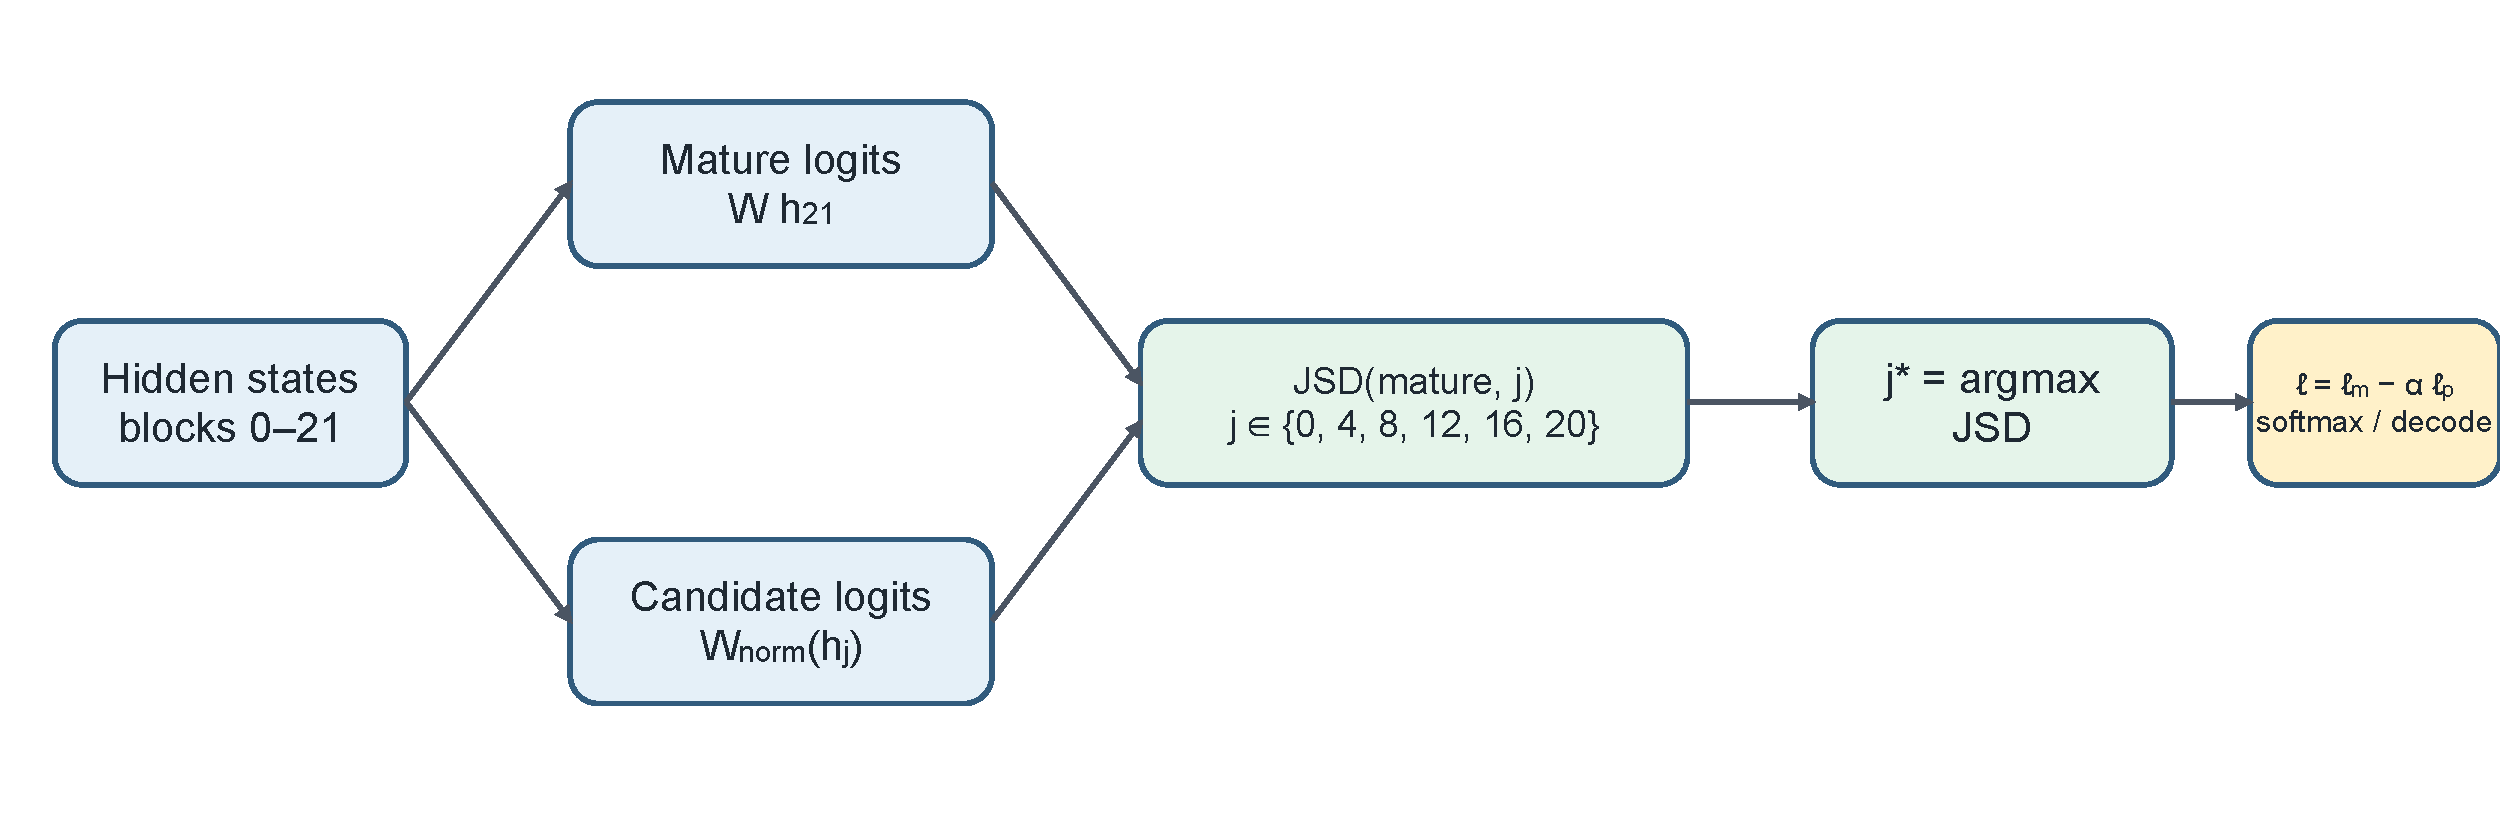
\includegraphics[width=\columnwidth]{Fig_2_DoLa_Workflow.pdf}\caption{DoLa workflow implemented in the active decoder.}\label{fig:dola}\end{figure}

\subsection{Active Epinet}
As shown in Fig.~\ref{fig:enn}, the active ENN concatenates two 2048-dimensional normalized representations. Each prior and learnable branch is an MLP with widths $4096\rightarrow512\rightarrow512\rightarrow(2048\times6)$, reshaped to $(2048,6)$ and contracted with $z$. The prior is frozen; only the learnable branch is optimized with AdamW. The recorded full-cache run uses 600 C4 documents, 56,515 token examples, a document-disjoint 90/10 split, batch size 32, learning rate $10^{-4}$, ten epochs, eight training $z$ samples, $\alpha=0.05$, weight decay $10^{-4}$, gradient clipping at 1.0, and a ReduceLROnPlateau scheduler. The best checkpoint is selected using validation loss.
\begin{figure}[t]\centering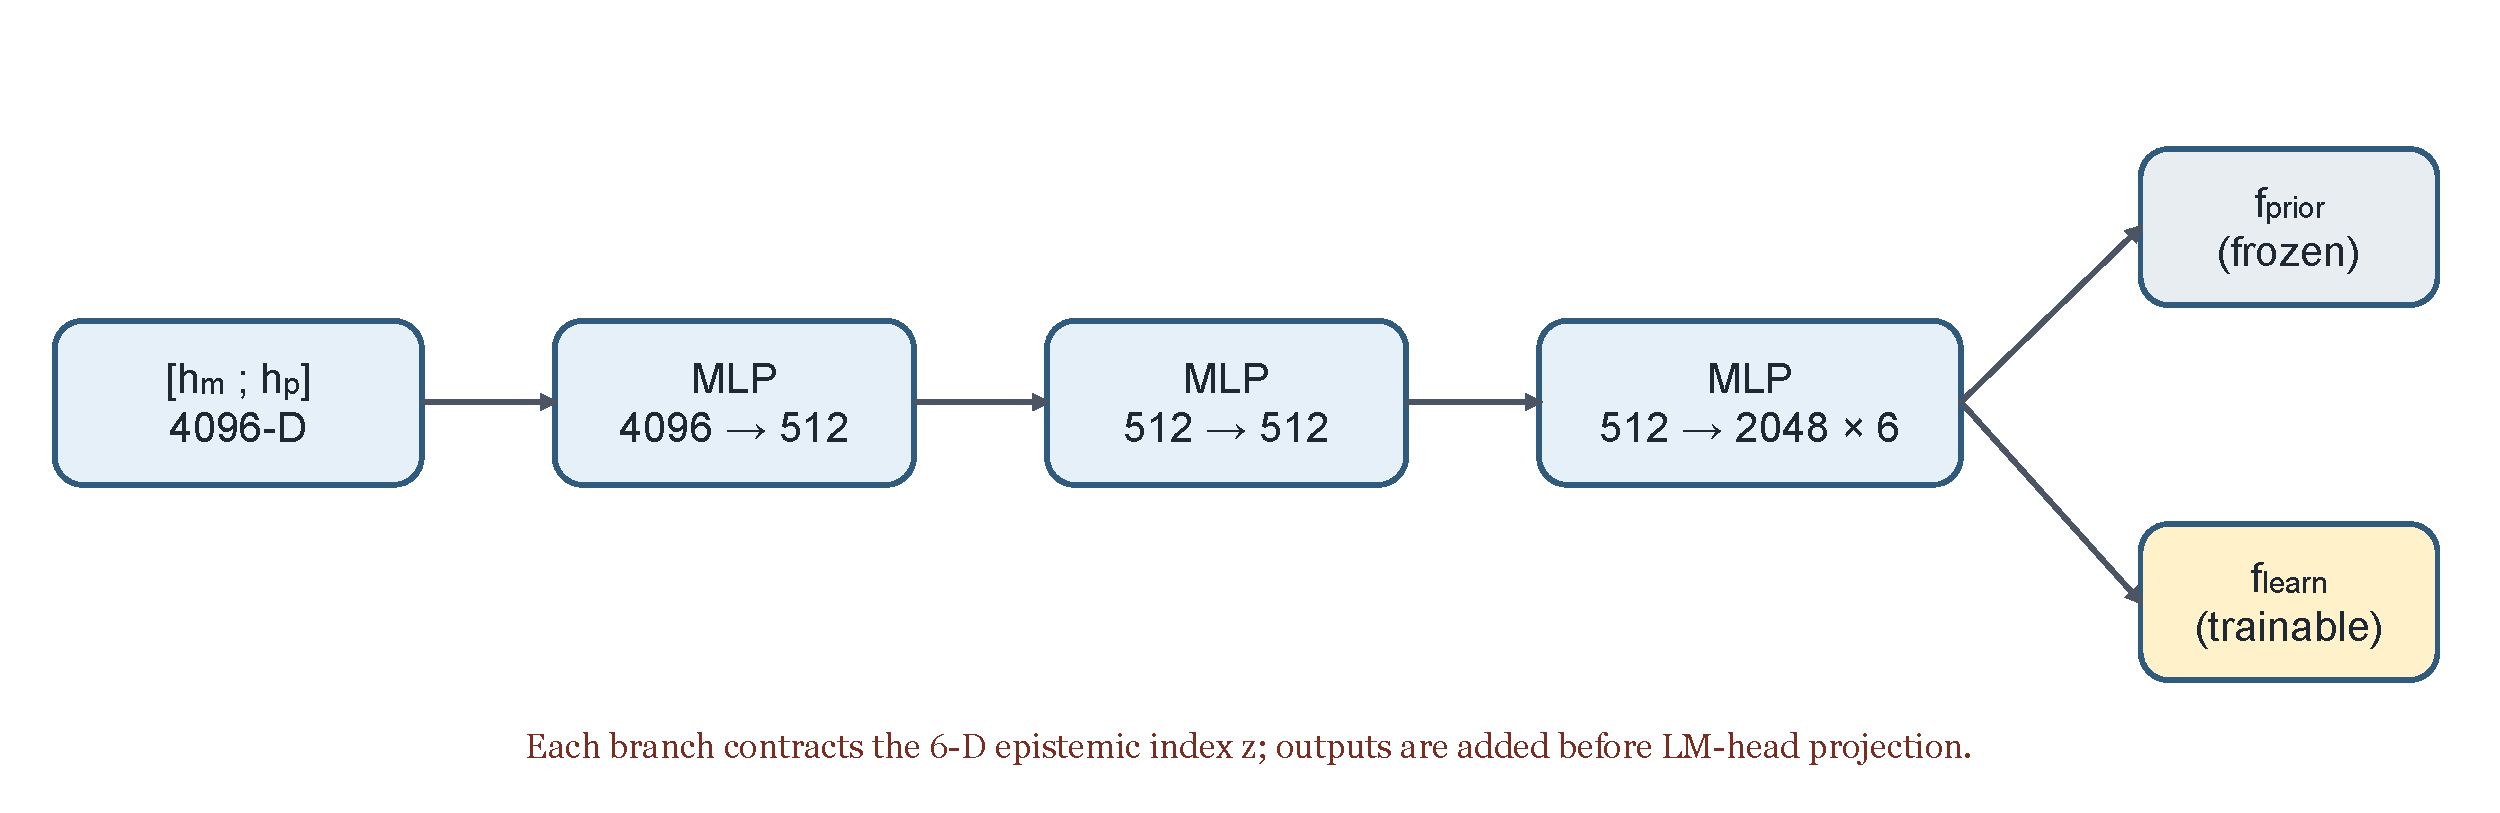
\includegraphics[width=\columnwidth]{Fig_3_Active_Epinet.pdf}\caption{Active C4-trained epinet. The epistemic index is sampled at each forward pass.}\label{fig:enn}\end{figure}

\subsection{Self-consistency and answer scoring}
The active runner samples DoLa candidates with temperature 0.7, top-$p$ 0.9, and a default limit of 16 new tokens. Plain self-consistency normalizes surface forms and selects by plurality. The ENN-weighted variant assigns candidate weight $c_i=\operatorname{clip}(1-H_i/\log|V|,0,1)$, where $H_i$ is the mean predictive entropy across the candidate. This quantity is an entropy-derived voting weight, not a calibrated probability. Fig.~\ref{fig:sc} summarizes the process.
\begin{figure}[t]\centering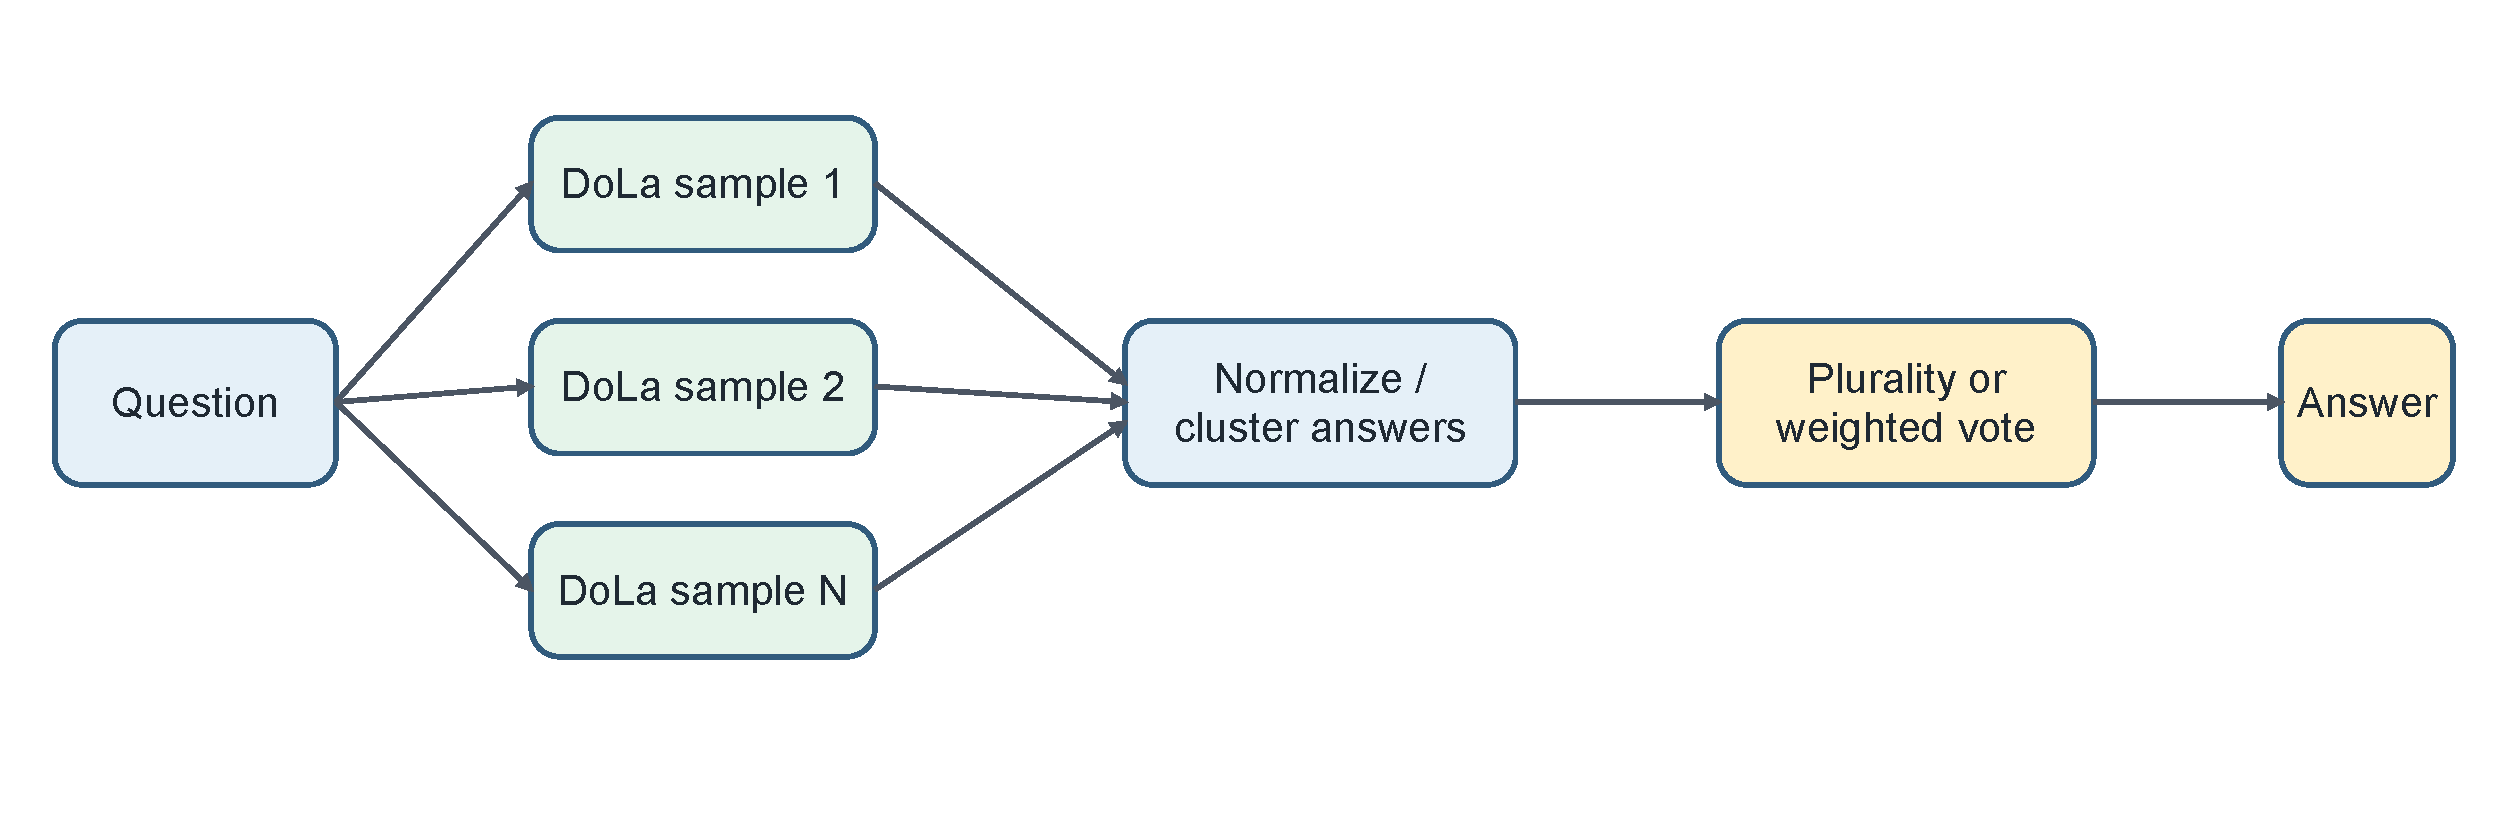
\includegraphics[width=\columnwidth]{Fig_4_Self_Consistency.pdf}\caption{Candidate generation and self-consistency aggregation.}\label{fig:sc}\end{figure}

\subsection{Detection versus mitigation}
The active interactive path can combine token statistics, semantic clustering, a prompted factuality judge, claim diagnostics, and a reliability head. The reliability head is a separate optional module requiring labeled answer-level examples; it is not trained by the C4 token ENN. The archived benchmark evaluates a supervised answer-correctness ENN and thresholded accept/reject decisions. Fig.~\ref{fig:detect} makes the distinction explicit.
\begin{figure}[t]\centering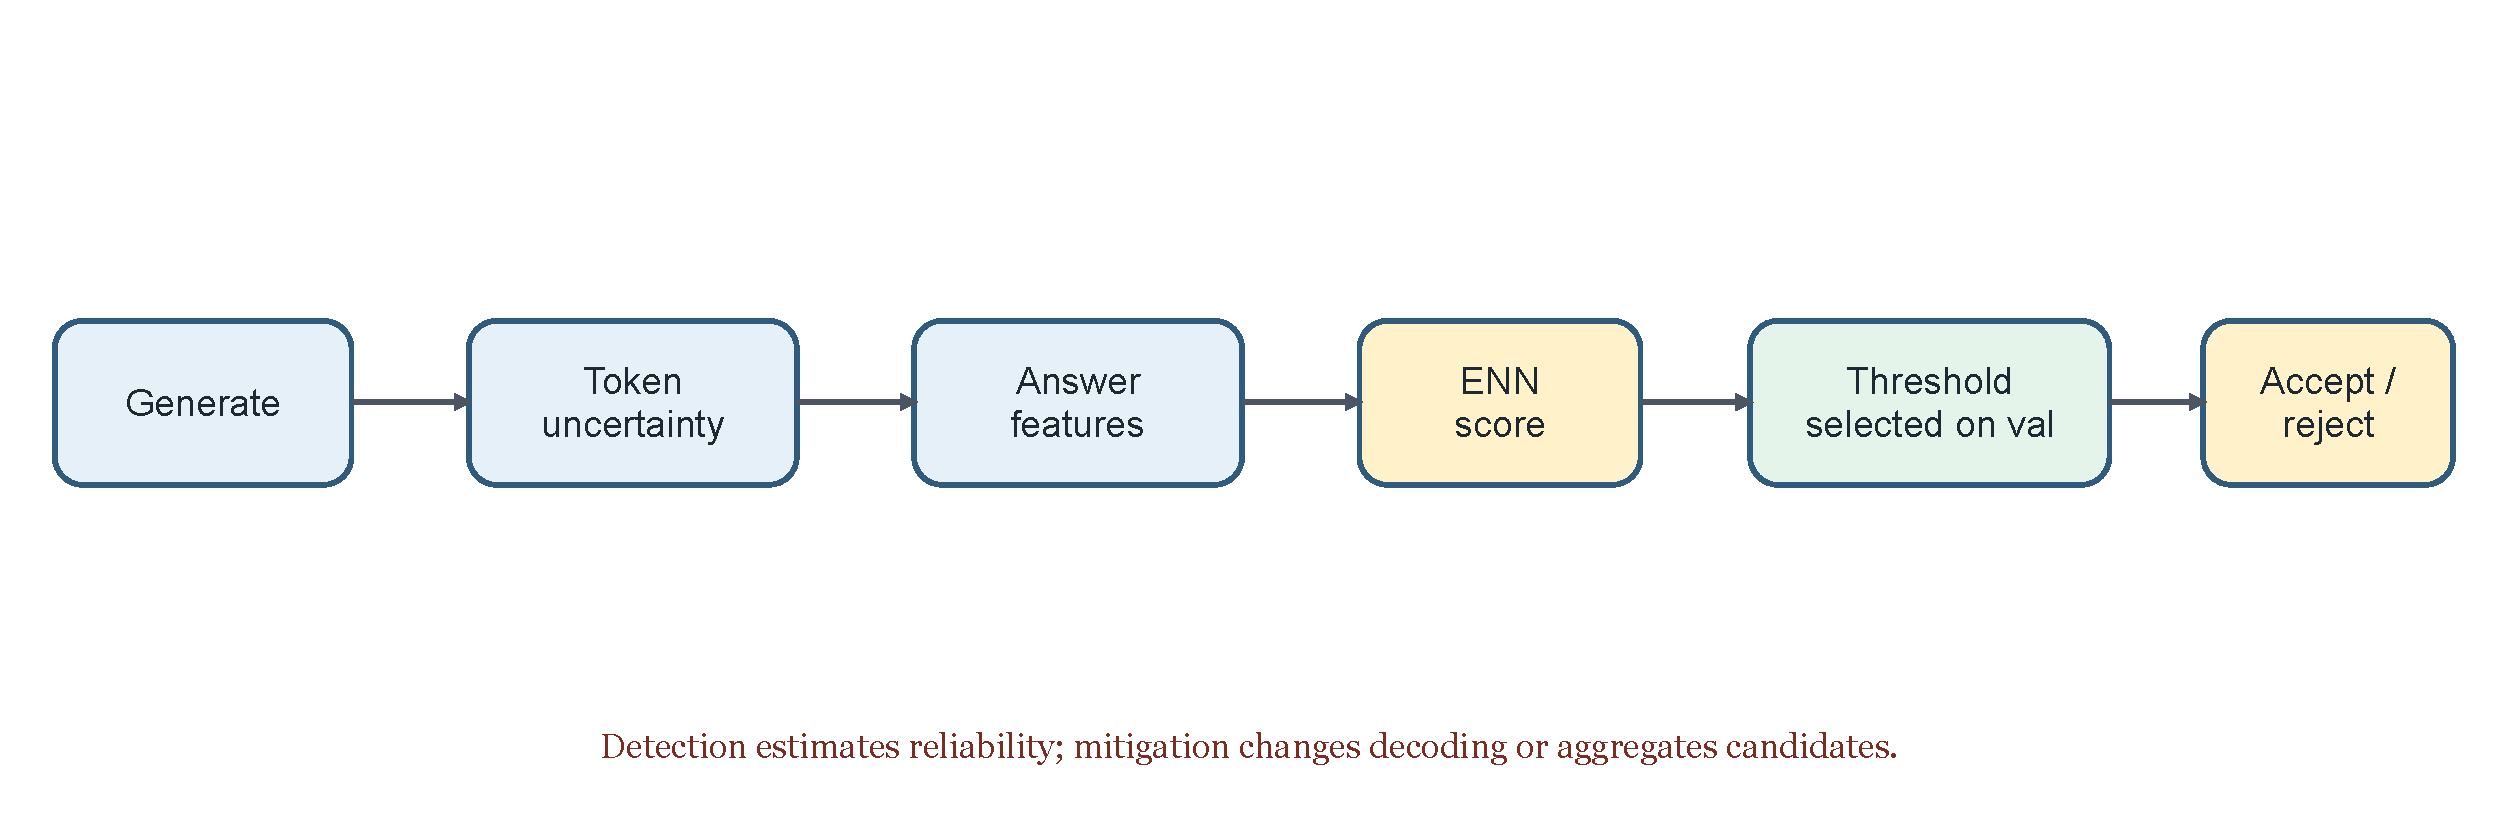
\includegraphics[width=\columnwidth]{Fig_5_Detection_Pipeline.pdf}\caption{Hallucination detection is a scoring and decision problem; mitigation acts on decoding or answer aggregation.}\label{fig:detect}\end{figure}

\begin{center}
\fbox{\begin{minipage}{0.94\columnwidth}
\textbf{Algorithm 1: Active inference and reliability-aware selection.}\\[2pt]
\footnotesize\ttfamily
Input: prompt q, frozen model M, optional ENN E, N candidates\\
1. Encode q with the TinyLlama chat template.\\
2. For i=1,...,N: decode Base or DoLa; if DoLa, select j* by (2).\\
3. If E is available, sample z and compute entropy diagnostics.\\
4. Normalize and cluster candidates; compute plurality/weighted votes.\\
5. If an answer detector is available, apply its validation threshold.\\
6. Return answer, decision, uncertainty, and provenance.
\end{minipage}}
\end{center}

\section{Experimental Setup}
\subsection{Repository artifacts and provenance}
Table~\ref{tab:env} records the active environment and saved artifacts. The model audit records Python 3.10.20, PyTorch 2.11.0, Transformers 5.17.0, Datasets 4.8.5, NumPy 1.26.4, and Apple Silicon MPS. The current requirements file declares compatible ranges but does not pin exact versions. The active cache is document-disjoint; the local ten-question file is too small to support a general factuality claim.

\begin{table}[t]\caption{Verified environment and artifact inventory}\label{tab:env}\centering\scriptsize\begin{tabular}{@{}p{.25\columnwidth}p{.70\columnwidth}@{}}\toprule
Item & Verified value / caveat\\\midrule
Base model & TinyLlama-1.1B-Chat-v1.0; 22 layers, hidden 2048, vocab 32,000\\
Runtime audit & Python 3.10.20; PyTorch 2.11.0; Transformers 5.17.0; Datasets 4.8.5; MPS\\
Active ENN data & C4 cache: 600 documents, 56,515 token examples; 90/10 document split\\
Active training & batch 32; 10 epochs; lr $10^{-4}$; $K=8$ train samples; $z$ dimension 6\\
Archived held-out set & 211 examples: 169 TruthfulQA + 42 HaluEval-QA; 54 positive, 157 negative\\
Saved models & active \code{checkpoints/enn\_best.pt}; archived V2/V3 checkpoints and reports\\
Reproducibility gap & archived upgraded trainer and evaluation source files are absent from checkout\\\bottomrule\end{tabular}\end{table}

\subsection{Archived benchmark protocol}
The archived report identifies the 211 examples as held out and states that feature normalization was fitted on training data only. It evaluates Base, DoLa, self-consistency, C4-trained ENN-V1, answer-correctness ENN-V2 variants, an ENN-V3 deep ensemble, and a complete combined architecture. Because the upgraded trainer source is missing, the results are presented as archived empirical evidence rather than as a fully reproducible execution of the active source tree. Threshold regimes were selected on validation data; the conservative regime prioritizes low FAR. Bootstrap intervals use paired resampling of held-out examples, and McNemar tests use paired predictions.

\section{Results}
\subsection{Quantitative comparison}
Table~\ref{tab:results} reports the main archived results. Base and DoLa have very high FAR, meaning most incorrect decisions are accepted under the selected policy. Self-consistency greatly improves accuracy and ECE relative to DoLa, but its recall for the positive class is only 0.389. The conservative DoLa+ENN operating point sharply reduces FAR to 0.038 and improves accuracy to 0.768, but recall falls to 0.204. This is useful for abstention-sensitive applications, not evidence of universal correctness improvement.

\begin{table*}[t]\caption{Archived held-out comparison on 211 examples, reported as percentages. Positive denotes the project-defined reliable/correct class; FAR is false acceptance of negative examples and FRR is false rejection of positives.}\label{tab:results}\centering\scriptsize\begin{tabular}{lrrrrrrrrrr}\toprule
Method & Acc. & Bal. Acc. & Prec. & Rec. & F1 & AUROC & AUPRC & ECE & FAR & FRR\\\midrule
Base TinyLlama (E0) & 28.4\% & 50.1\% & 25.6\% & 94.4\% & 40.3\% & 55.4\% & 40.2\% & 45.8\% & 94.3\% & 5.6\%\\
TinyLlama + DoLa (E5) & 29.9\% & 48.6\% & 25.0\% & 87.0\% & 38.8\% & 57.1\% & 40.6\% & 39.5\% & 89.8\% & 13.0\%\\
DoLa + SC (E6) & 65.4\% & 56.7\% & 34.4\% & 38.9\% & 36.5\% & 57.1\% & 40.6\% & 20.7\% & 25.5\% & 61.1\%\\
DoLa + ENN-V2 (E5b) & 76.8\% & 58.3\% & 64.7\% & 20.4\% & 31.0\% & 61.8\% & 39.3\% & 12.3\% & 3.8\% & 79.6\%\\
DoLa + ENN-V2 + SC (E7) & 76.8\% & 58.3\% & 64.7\% & 20.4\% & 31.0\% & 61.8\% & 39.3\% & 12.3\% & 3.8\% & 79.6\%\\
2048-D ENN alone (E2-B) & 78.2\% & 60.4\% & 72.2\% & 24.1\% & 36.1\% & 69.1\% & 51.3\% & 11.6\% & 3.2\% & 75.9\%\\
Complete combined & 72.5\% & 62.7\% & 46.0\% & 42.6\% & 44.2\% & 67.0\% & 44.8\% & 19.5\% & 17.2\% & 57.4\%\\\bottomrule\end{tabular}\end{table*}

Fig.~\ref{fig:performance} visualizes the archived accuracy comparison. The strongest AUROC and AUPRC come from the 2048-D representation-only ENN, not the complete combined architecture. This is an important negative result: more components did not monotonically improve ranking quality.
\begin{figure}[t]\centering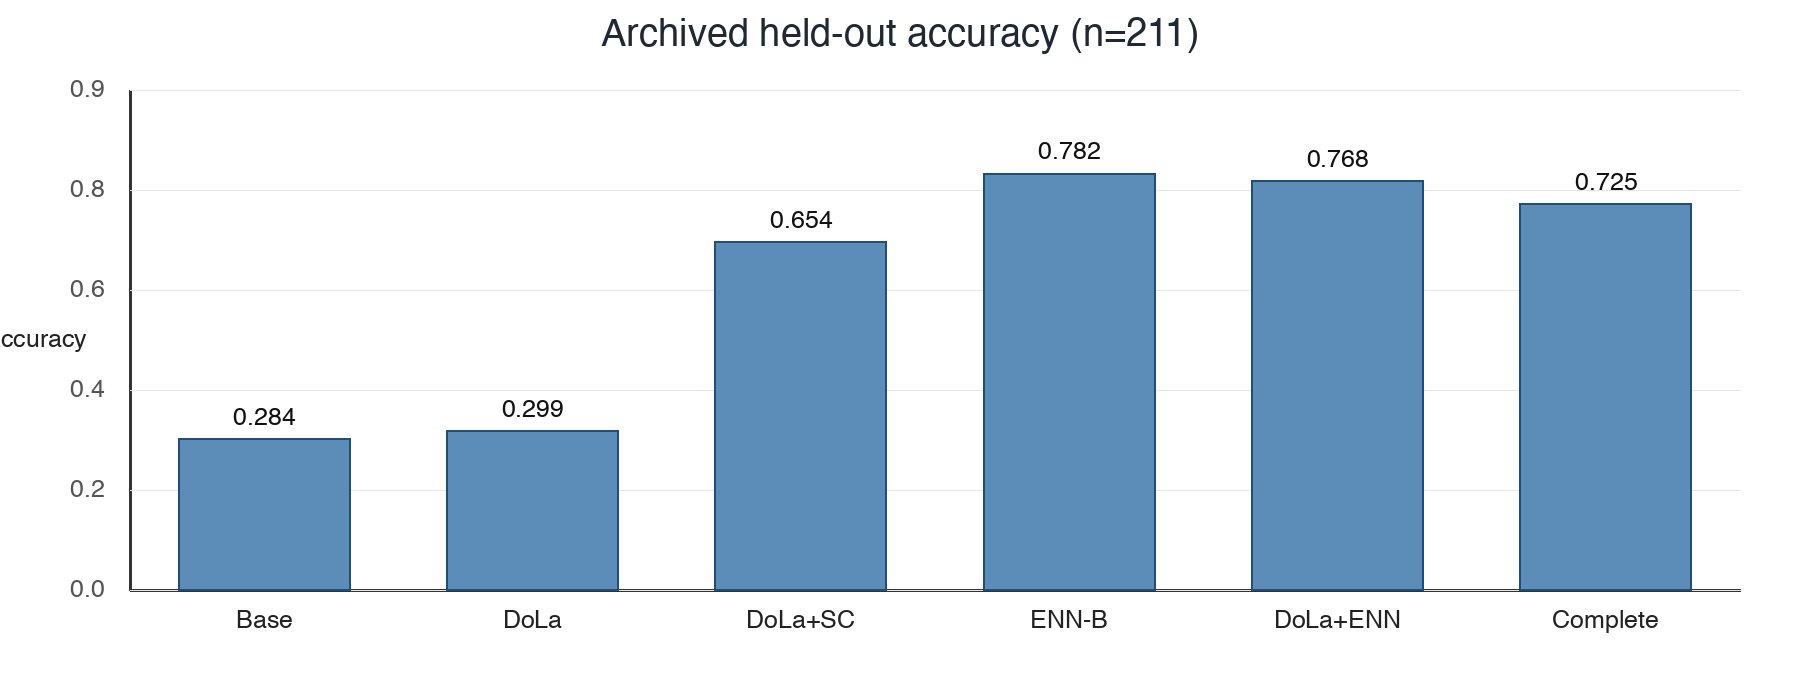
\includegraphics[width=\columnwidth]{fig6_performance.png}\caption{Archived accuracy comparison across evaluated architectures.}\label{fig:performance}\end{figure}

\subsection{Ablation}
The archived feature ablation found AUROC 0.6681 for the 2048-D representation alone, 0.3664 for eight token diagnostics alone, 0.5758 for six self-consistency features alone, 0.6695 for representation plus token diagnostics, and 0.6713 for the full feature set. The representation therefore carries most of the discriminative signal. Adding all self-consistency features reduced accuracy from 0.7488 to 0.7346 while increasing AUROC by only 0.0032. This pattern agrees with the E5b--E7 comparison, for which the saved decisions are identical. Fig.~\ref{fig:ablation} is an audit visualization of a held-out result; it does not establish that every source component is currently executable.
\begin{figure}[t]\centering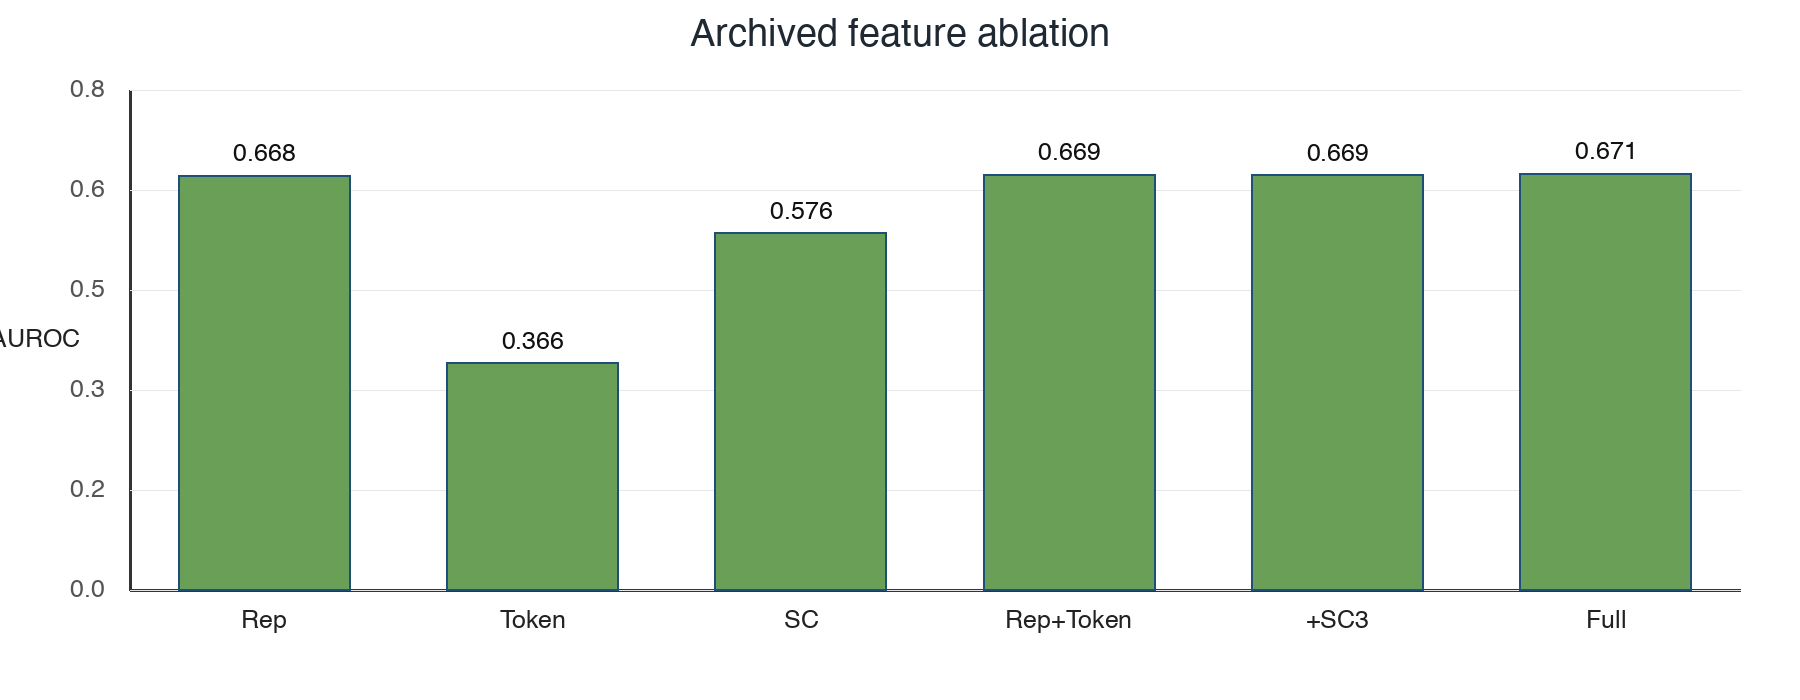
\includegraphics[width=\columnwidth]{fig7_ablation.png}\caption{Archived ENN feature ablation visualization.}\label{fig:ablation}\end{figure}

\subsection{Statistical analysis and operating points}
For E5b versus DoLa, paired bootstrap accuracy delta was 0.4692 with 95\% CI [0.3762, 0.5556], and McNemar's test reported $p<0.001$. For the complete architecture versus E5b, the accuracy delta was -0.0427 with 95\% CI [-0.1043, 0.0099] and McNemar's $p=0.163$, so the apparent difference is not statistically significant in this audit. Across saved seeds, the reported complete-architecture accuracy was $0.7611\pm0.0023$, F1 $0.3668\pm0.0101$, and AUROC $0.6351\pm0.0010$. These repeated-run statistics are useful but inherit the benchmark's fixed sample and missing-source limitations.

\subsection{Case and confusion analysis}
The conservative E7 confusion matrix is TP=11, TN=151, FP=6, FN=43 (Fig.~\ref{fig:cm}). It is a high-specificity detector: only six negative examples are accepted, but 43 positive examples are rejected. This makes the system suitable for a workflow that can abstain and request verification, but unsuitable as a standalone answer generator. The archived raw predictions should be used for claim-level case studies; no individual example is quoted here because the report package does not preserve a stable human-readable case-study table with provenance.
\begin{figure}[t]\centering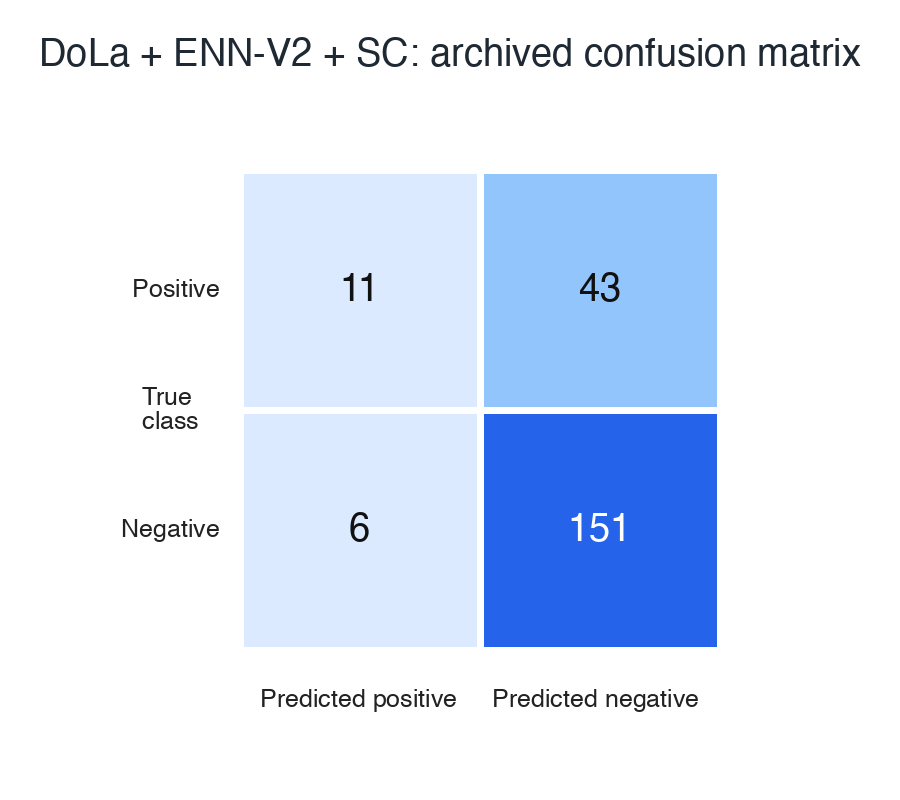
\includegraphics[width=.9\columnwidth]{fig8_confusion.png}\caption{Archived reliability visualization for the upgraded benchmark; the accompanying confusion counts are TP=11, TN=151, FP=6, FN=43 for E7.}\label{fig:cm}\end{figure}

\section{Discussion}
The comparison reveals three distinct effects. First, DoLa alone barely changes archived decision accuracy relative to Base and leaves FAR above 0.89. Second, self-consistency substantially changes the operating behavior: accuracy rises to 0.654 and ECE falls to 0.207, while positive-class recall falls to 0.389. Third, the answer-correctness ENN yields the strongest conservative rejection behavior and the best ranking in its representation-only form. Adding self-consistency does not improve the E5b operating point because the saved E5b and E7 decisions are identical.

The active C4-trained epinet cannot be credited with the archived answer-level results. Its training loss is next-token cross-entropy, and the default ENN logit weight in \code{config.yaml} is zero. In the active runner, predictive entropy affects a candidate weight but is not converted into a calibrated correctness probability. The archived upgrade addresses this objective mismatch by training on answer-level correctness, but its source is absent. For that reason, the paper keeps the active system description and archived benchmark results separate rather than presenting them as one executable architecture.

The low FAR / high FRR operating point is a practical trade-off, not a free improvement. Class imbalance is substantial (157 negatives versus 54 positives), so accuracy alone is misleading: an always-reject baseline reaches 0.744 accuracy while detecting no positives. AUROC, AUPRC, balanced accuracy, FAR, FRR, and risk--coverage curves are therefore necessary. Calibration is also operating-point dependent; ECE 0.123 is encouraging, but it does not imply that every score is a probability of truth.

\section{Limitations and Future Work}
The most important limitation is provenance: the archived MC-dropout/deep-ensemble trainer, feature construction, and threshold-selection code is not in the active repository. Reproducing those numbers requires recovering the missing source or rerunning the experiment from a preserved commit. The active local QA file has only ten questions, and the C4 feature cache does not preserve complete source-document provenance or per-token selected layers. Exact software versions are recorded in audit reports but are not pinned in the requirements file.

The 211-example benchmark is imbalanced and combines two datasets. The project should archive the positive/negative label semantics, prompt templates, and exact thresholding code alongside the predictions. Future work should: (i) restore the upgraded source and commit hashes; (ii) create question-disjoint train/validation/test partitions; (iii) fit calibration and thresholds only on validation data; (iv) evaluate full TruthfulQA and HaluEval protocols plus a fresh domain-shift set; (v) report repeated seeds and confidence intervals; (vi) compare calibrated abstention against retrieval and verifier baselines; and (vii) measure end-to-end latency and memory on the target hardware. A stronger active ENN should be trained directly on answer correctness or claims, while C4 token prediction remains a separate language-model diagnostic.

\section{Conclusion}
This paper documents a TinyLlama reliability pipeline that combines layer-contrastive decoding, epistemic sampling, and self-consistency while separating hallucination detection from mitigation. The active source implements DoLa and a C4-trained epinet with explicit uncertainty diagnostics. The archived benchmark offers stronger, but not fully reproducible, evidence for answer-level reliability: a 2048-D ENN reaches AUROC 0.691, and a conservative DoLa+ENN operating point reaches accuracy 0.768 with FAR 0.038 at the cost of recall 0.204. Self-consistency does not alter that operating point, and the complete combined architecture is not significantly better than DoLa+ENN. The supported conclusion is conditional: the project demonstrates an abstention-oriented reliability workflow, not a universal hallucination-prevention method. Recovering the missing source and validating on larger, balanced, question-disjoint datasets are prerequisites for stronger publication claims.

\section*{Acknowledgment}
The authors acknowledge the guidance of Palacharla Ravi Kumar, Assistant Professor Sr. Grade-2, SCOPE, VIT-AP University.

\bibliographystyle{IEEEtran}
\bibliography{references}
\end{document}
